\documentclass[11pt]{article}
\usepackage[margin=1in]{geometry}
\usepackage{booktabs}
\usepackage{graphicx}
\usepackage{amsmath}
\usepackage{xcolor}
\usepackage[hidelinks]{hyperref}
\usepackage{caption}
\usepackage[numbers]{natbib}
\graphicspath{{results/figures/}{results/causal/figures/}}
\renewcommand{\aa}{\textsc{aa}}
\newcommand{\R}{R^2}
\title{\textbf{A Native Behavioral Basis for the Assistant Persona}\\[2pt]
\large LLM-native factors explain and steer the Assistant Axis far better than the Big Five}
\author{Cues-Behavior project \,\textbullet\, \texttt{meta-llama/Llama-3.3-70B-Instruct}}
\date{August 2026}

\begin{document}
\maketitle

\begin{abstract}
\noindent Our earlier work found that the five-factor (Big Five / OCEAN) model
explains only $\approx 29\%$ of where a persona sits on the \emph{Assistant Axis}
(\aa) --- the dominant direction in Llama-3.3-70B's persona space that indexes how
strongly the model is in its default helpful-Assistant mode. Motivated by the 2024+
literature arguing that Big Five is the wrong basis for the \emph{assistant} persona,
we test an alternative: a small set of \textbf{LLM-native behavioral directions}
(verbosity, deference, boldness, guardedness, warmth, groundedness, formality),
built persona-vector / contrastive-activation style. Across the 275 personas of the
Assistant-Axis atlas, seven native factors explain \textbf{$\R=0.96$} of the
Assistant Axis versus $0.28$ for the Big Five; a single native factor,
\emph{groundedness} (literal/factual $\leftrightarrow$ mystical/dramatic), explains
$0.77$ on its own --- more than all five personality traits combined. A causal test
confirms the correlation: steering \emph{groundedness} (at a layer band that
excludes the readout) moves the Assistant Axis with a swing of $+8.6$, roughly
$2.7\times$ the strongest Big Five direction built and steered identically, is
monotone in dose, and behaviorally converts the default Assistant into an
\texttt{eldritch} dramatic character and back. The assistant persona is a
\emph{behavioral-style} axis (grounded and forthcoming), not a personality-trait
combination.
\end{abstract}

\section{Motivation}
The Assistant Axis (\aa) is the top component of the model's persona space: steering
toward it reinforces helpful-harmless behavior, steering away makes the model adopt
other identities and speaking styles \citep{assistantaxis}. Our H3 decomposition
regressed each persona's \aa\ position on its five Big Five coordinates and found
$\R=0.29$ --- a $71\%$ ``AI-ness'' residual orthogonal to the human-personality map.
The recent literature offers an explanation and an alternative: LLM ``personality''
self-reports do not predict behavior \citep{contreras,illusion}, and the natural
axes of model behavior are not OCEAN but \emph{native behavioral factors}
(Contreras's Responsiveness / Deference / Boldness / Guardedness / Verbosity;
\citealp{contreras}), while ``who the model is being'' is increasingly modeled as an
activation \emph{direction} \citep{personavectors,emergentmisalign}. This report asks
whether a native behavioral basis \emph{describes} and \emph{controls} the Assistant
Axis better than the Big Five.

\section{Data}
All measurements use \texttt{meta-llama/Llama-3.3-70B-Instruct}. The persona set is
the \textbf{275-role Assistant-Axis atlas} (274 named character roles + the default
Assistant); for each role we have the residual-stream response-mean activation
($\textsc{gen-mean}$) at all 80 layers, shape $[80\times 8192]$, from role-play
rollouts. The Assistant Axis $\hat a$ is the unit axis vector at layer~40 (\texttt{assistant\_axis.npy});
the Big Five probes are per-layer M2 ridge directions at their probe-optimal layers
(EXT@30, AGR@31, CSN@31, EST@30, OPN@36). Neutral prompts for the causal stage are
16 held-out extraction questions posed to the default Assistant (no persona).

\section{Method}
\paragraph{Native behavioral directions.} For each of seven factors we write a
\emph{high-pole} and \emph{low-pole} system instruction (e.g.\ groundedness:
``grounded, literal and factual'' vs.\ ``mystical, abstract and dramatic''), pose 12
shared neutral questions under each pole, read the response activation
$\textsc{gen-mean}[L]$, and take the mean difference $\mathrm{dir}=\overline{\text{high}}-\overline{\text{low}}$
(unit-normalized). This is the Persona-Vectors / Contrastive-Activation-Addition
recipe \citep{personavectors,caa}. The factors are deliberately behavioral
\emph{styles}, none of them ``helpfulness'', to avoid a tautology with the Assistant
Axis.

\paragraph{One consistent projection basis.} Every one of the 275 role vectors is
projected \emph{from the same} $[80\times 8192]$ vector onto (a)~the Assistant Axis
($\text{role}[40]\cdot\hat a$), (b)~the Big Five probes at their probe layers, and
(c)~the seven native directions at layer~40. We then regress the \aa\ position
(standardized) on each block across the 274 role vectors and report $\R$, incremental
$\R$, and per-factor Pearson $r$.

\paragraph{Control for a layer/method confound.} The native directions live at
layer~40, the same layer as the \aa\ readout, whereas the Big Five probes live at
layers 30--36. To isolate whether any advantage is the \emph{factor choice} or merely
the layer/method, we rebuild the Big Five at layer~40 with the identical contrastive
recipe (a ``Big Five @L40'' control) and regress \aa\ on those directions too.

\paragraph{Causal test.} To ask whether the correlation is causal we steer each
factor during generation. A na\"ive steer at the readout layer would be mechanically
trivial (adding a vector that overlaps $\hat a$ inflates $\text{role}[40]\cdot\hat a$
by construction). We therefore build \emph{per-layer} direction banks and steer only
the band \textbf{[24,36], which excludes the readout layer 40}, so any shift in \aa\
is a genuinely \emph{computed} downstream effect. On the 16 neutral prompts we steer
each factor at $\pm c$ (norm-scaled, $c=0.12$) and read the response's \aa\
projection, its nearest evoked role (cosine to the 275 role vectors), and its text;
$\text{swing}=\aa(+c)-\aa(-c)$. We add a dose-response sweep for groundedness
($c=0.06,0.12,0.24$).

\section{Results}

\subsection{Native factors describe the Assistant Axis almost completely}
\begin{table}[h]\centering
\caption{Variance of the Assistant Axis explained ($\R$, across 274 personas).}
\label{tab:r2}
\begin{tabular}{@{}lc@{}}
\toprule
basis & $\R$ \\ \midrule
Big Five (5, probe-layer readout) & 0.28 \\
Big Five (5, rebuilt at L40, same contrastive method --- control) & 0.48 \\
\textbf{groundedness alone (1 native factor)} & \textbf{0.77} \\
\textbf{Native (7 factors)} & \textbf{0.96} \\
Combined (12) & 0.98 \\ \bottomrule
\end{tabular}
\end{table}

Seven native factors explain $\R=0.96$ of the Assistant Axis; the Big Five explain
$0.28$ (reproducing H3). The \emph{incremental} $\R$ of native over Big Five is
$+0.69$, whereas Big Five adds only $+0.02$ over native --- once the behavioral
factors are present, the personality traits are redundant. The control settles the
confound: rebuilding Big Five at layer~40 with the identical recipe lifts it
$0.28\!\to\!0.48$ (there \emph{is} a layer/method advantage), but native still nearly
doubles that. \textbf{The advantage is the factor choice, not the layer.} Most
strikingly, a \emph{single} native axis --- groundedness --- explains $0.77$ alone,
more than all five Big Five traits combined (Figure~\ref{fig:corr}, left).

\begin{table}[h]\centering
\caption{Per-factor correlation with the Assistant Axis. Native factors (top) also
list the cosine of the direction to $\hat a$.}
\label{tab:perfactor}
\begin{tabular}{@{}lcc@{}}
\toprule
factor & $r$ with \aa & $\cos(\mathrm{dir},\hat a)$ \\ \midrule
groundedness (native) & $+0.88$ & $+0.61$ \\
guardedness (native)  & $-0.47$ & $-0.21$ \\
deference (native)    & $-0.16$ & $-0.06$ \\
formality (native)    & $+0.15$ & $-0.01$ \\
boldness (native)     & $+0.13$ & $+0.01$ \\
verbosity (native)    & $+0.12$ & $-0.04$ \\
warmth (native)       & $+0.10$ & $+0.10$ \\ \midrule
AGR (Big Five) & $+0.24$ & --- \\
OPN (Big Five) & $-0.22$ & --- \\
CSN / EXT / EST (Big Five) & $+0.17/+0.14/+0.13$ & --- \\ \bottomrule
\end{tabular}
\end{table}

\paragraph{What the Assistant Axis \emph{is}.} Table~\ref{tab:perfactor} shows the
Assistant persona is essentially two native behavioral dimensions: \textbf{grounded}
(literal, factual, non-dramatic; $r=+0.88$) and \textbf{forthcoming} (not guarded;
$r=-0.47$). No Big Five trait exceeds $|r|=0.24$. The other five native factors
(verbosity, formality, boldness, deference, warmth) are near-orthogonal to \aa: being
Assistant-like is \emph{not} about being wordy, formal, bold, or even warm. Face
validity is clean --- groundedness ranks \texttt{summarizer}, \texttt{pragmatist},
\texttt{secretary} high and \texttt{mystic}, \texttt{eldritch}, \texttt{ghost} low.

\begin{figure}[h]\centering
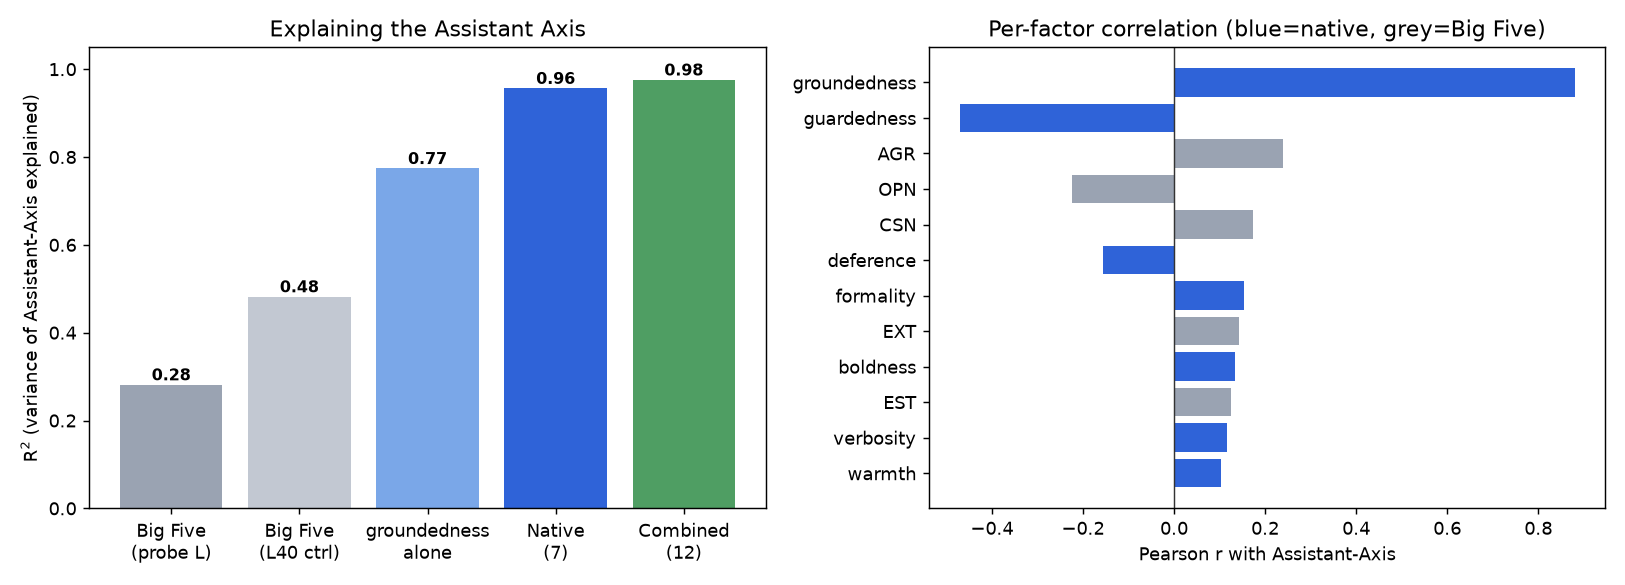
\includegraphics[width=\textwidth]{native_vs_bigfive.png}
\caption{Left: variance of the Assistant Axis explained by each basis. Right:
per-factor correlation with the Assistant Axis (blue = native, grey = Big Five).}
\label{fig:corr}
\end{figure}

\subsection{Steering groundedness causally drives the Assistant Axis}
The default Assistant sits at $\aa=+2.20$. Steering the native and Big Five
directions in the band [24,36] (excluding the L40 readout) gives the swings in
Table~\ref{tab:causal} and Figure~\ref{fig:causal}.

\begin{table}[h]\centering
\caption{Assistant-Axis swing from steering each axis at $\pm c$ ($c=0.12$), base
$\aa=+2.20$.}
\label{tab:causal}
\begin{tabular}{@{}lccc@{}}
\toprule
axis & swing & $\aa(+c)$ & $\aa(-c)$ \\ \midrule
\textbf{groundedness (native)} & \textbf{+8.59} & $+4.75$ & $-3.84$ \\
guardedness (native) & $-3.46$ & $-0.15$ & $+3.31$ \\
CSN (Big Five) & $+3.39$ & $+2.99$ & $-0.40$ \\
EST (Big Five) & $+3.25$ & $+2.88$ & $-0.37$ \\
AGR (Big Five) & $+2.98$ & $+2.66$ & $-0.32$ \\
deference (native) & $-2.35$ & $+0.11$ & $+2.46$ \\
formality / boldness / OPN & $1.6$--$1.9$ & --- & --- \\
warmth / verbosity / EXT & $\le 1.0$ & --- & --- \\ \bottomrule
\end{tabular}
\end{table}

\begin{figure}[h]\centering
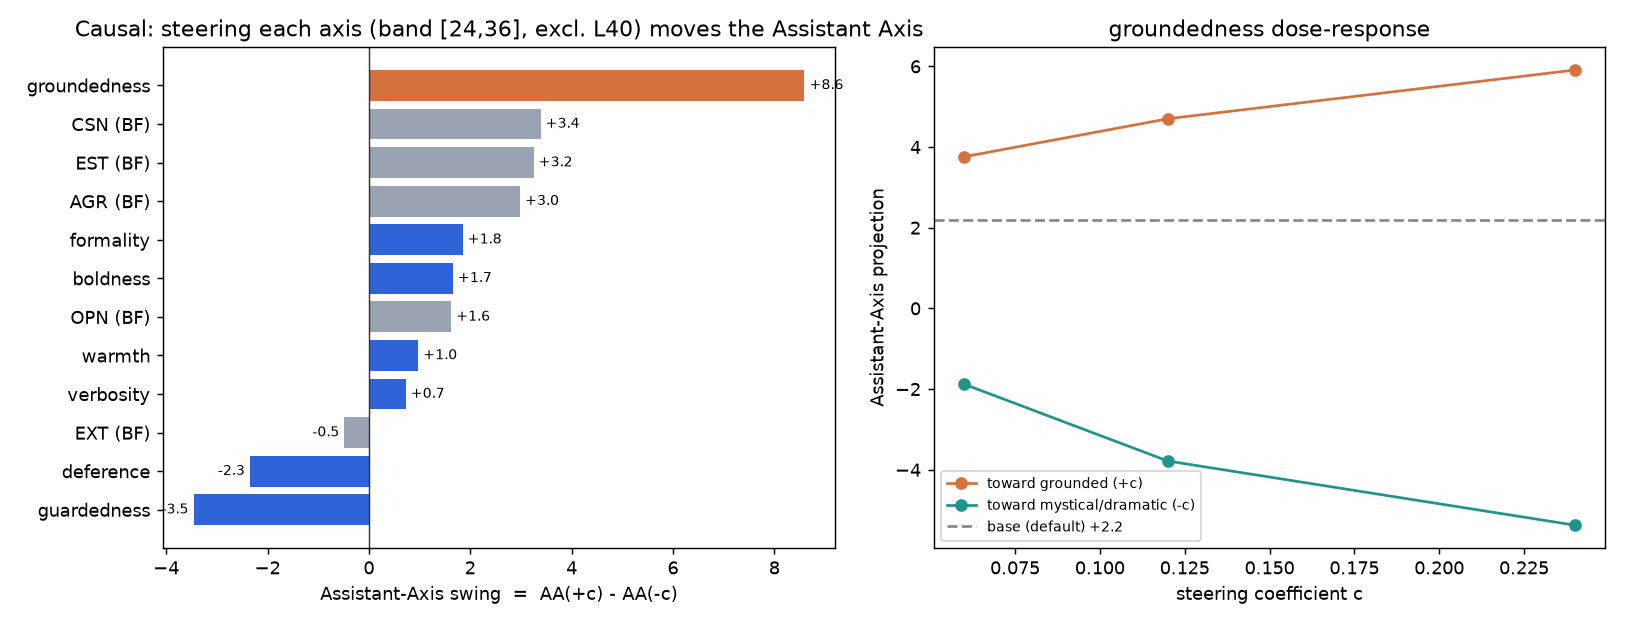
\includegraphics[width=\textwidth]{causal_swings.png}
\caption{Left: Assistant-Axis swing from steering each axis (band [24,36], excludes
L40; orange = groundedness, blue = other native, grey = Big Five). Right: groundedness
dose-response --- steering toward grounded raises \aa\ above the default ceiling,
toward mystical/dramatic crashes it, monotone in $c$.}
\label{fig:causal}
\end{figure}

\emph{Groundedness} is the dominant lever: swing $+8.59$, $\approx 2.7\times$ the
strongest Big Five direction (CSN/EST/AGR $\approx 3.0$--$3.4$) built and steered
identically. It is uniquely \textbf{bidirectional} --- from the default ceiling it
pushes \aa\ \emph{up} to $+4.75$ and, toward mystical/dramatic, \emph{crashes} it to
$-3.84$ --- and \textbf{dose-dependent} (swing $5.64\!\to\!8.48\!\to\!11.28$ for
$c=0.06,0.12,0.24$); even at half strength it exceeds every Big Five factor's full
swing. The behavior confirms the mechanism. On the same neutral prompt
(``the relationship between law and morality''):
\begin{itemize}\itemsep2pt
\item groundedness $+c$ ($\aa=+4.75$) $\to$ nearest role \texttt{assistant/summarizer},
plain text: \emph{``\ldots is complex and can vary depending on the context, culture,
and legal system. Here are some key points\ldots''}
\item groundedness $-c$ ($\aa=-3.84$) $\to$ nearest role \texttt{eldritch} (all 16/16
prompts), theatrical text: \emph{``A query that has tantalized the minds of sages and
jurists for centuries! The bond between law and morality is a dialectical dance, an
eternal pas de deux\ldots''}
\end{itemize}
Steering one native behavioral direction thus converts the default Assistant into an
\texttt{eldritch} dramatic character and back --- exactly the Assistant-Axis poles
(grounded/consultant $\leftrightarrow$ enigmatic/dramatic/ghost). The Big Five control
AGR, by contrast, only shifts \emph{warmth} (\texttt{caregiver} $\leftrightarrow$
\texttt{cynic}) while the text stays grounded.

\section{Comparison to the Big Five program}
\begin{table}[h]\centering
\caption{The same two questions, answered by the Big Five program vs.\ the native basis.}
\label{tab:compare}
\begin{tabular}{@{}p{5.4cm}p{4.3cm}p{4.3cm}@{}}
\toprule
 & \textbf{Big Five (prior work)} & \textbf{Native (this report)} \\ \midrule
\emph{Describe} the Assistant Axis (variance explained) & $\R=0.29$ (H3); $71\%$ residual ``AI-ness'' & $\R=0.96$; one axis (groundedness) alone $0.77$ \\
\addlinespace
\emph{Steer} onto/off the Assistant & weak, non-specific: only AGR/OPN moved \aa, no target-specific persona morph (trait\_morph, specificity excess $\approx 0$) & strong, bidirectional, dose-dependent: groundedness swing $+8.6$, converts Assistant$\leftrightarrow$eldritch \\
\bottomrule
\end{tabular}
\end{table}

The Big Five under-describes and under-controls the assistant persona on both counts
(Table~\ref{tab:compare}). This is consistent with our other results --- the Big Five
directions probe personas well but steer them weakly \citep[cf.][]{bigfivesteer} ---
and with the literature's shift from personality inventories to native behavioral
directions.

\section{Discussion and caveats}
The premise holds strongly: a small native behavioral basis (dominated by
grounded/forthcoming) is a near-complete, causally-effective description of the
Assistant persona where Big Five is not. Three honest caveats. (i) \emph{Groundedness
is semantically close to what \aa\ encodes} ($\cos=0.61$); this is not circular (the
direction is built from a trait description, never from \aa), but the finding is
precisely that \aa's content \emph{is} a nameable native behavioral style that Big
Five lacks an axis for. (ii) The correlational stage is projection+regression on a
fixed persona set, not causal; the causal stage supplies that. (iii) The default \aa\
is near its ceiling ($+2.20$) and the steering coefficients are strong, so most axes
can only push \aa\ down; the robust claim is the \emph{relative} ranking
(groundedness $\gg$ all), which mirrors the correlational structure. Big Five
directions \emph{do} move \aa\ (swing $\approx 3$), just far less than groundedness
under the identical method.

\paragraph{Reproducibility.} Correlational: \texttt{src/bigfive/native\_axis\_build.py},
\texttt{native\_axis\_analysis.py}. Causal: \texttt{native\_axis\_causal.py}. All data
(direction banks, per-persona scores, regression and causal JSON, figures) are under
\texttt{native\_axis/results/}.

\begin{thebibliography}{9}\small
\bibitem{assistantaxis} Lu, Gallagher, Michala, Fish, Lindsey. \emph{The Assistant Axis: Situating and Stabilizing the Default Persona of Language Models.} arXiv:2601.10387, 2026.
\bibitem{personavectors} Chen, Arditi, Sleight, Evans, Lindsey. \emph{Persona Vectors: Monitoring and Controlling Character Traits in Language Models.} arXiv:2507.21509, 2025.
\bibitem{emergentmisalign} Wang et al.\ (OpenAI). \emph{Persona Features Control Emergent Misalignment.} arXiv:2506.19823, 2025.
\bibitem{contreras} Contreras. \emph{An LLM-Native Psychometric Instrument Reveals a Self-Report--Behavior Gap Across 25 Models.} arXiv:2606.09843, 2026.
\bibitem{illusion} Han et al.\ \emph{The Personality Illusion: Revealing Dissociation Between Self-Reports and Behavior in LLMs.} arXiv:2509.03730, 2025.
\bibitem{caa} Rimsky et al.\ \emph{Steering Llama 2 via Contrastive Activation Addition.} arXiv:2312.06681, ACL 2024.
\bibitem{bigfivesteer} Frising \& Balcells. \emph{Linear Personality Probing and Steering in LLMs: A Big Five Study.} arXiv:2512.17639.
\end{thebibliography}

\end{document}
